\documentclass[tikz]{standalone}%

\usepackage[utf8]{inputenx}%  http://ctan.org/pkg/inputenx
% Euler for math | Palatino for rm | Helvetica for ss | Courier for tt
\renewcommand{\rmdefault}{ppl}% rm
\linespread{1.05}% Palatino needs more leading
\usepackage[scaled]{helvet}% ss //  http://ctan.org/pkg/helvet
\usepackage{courier}% tt // http://ctan.org/pkg/courier
\usepackage{eulervm}  %  http://ctan.org/pkg/eulervm
% a better implementation of the euler package (not in gwTeX)
\normalfont%
\usepackage[T1]{fontenc}%  http://ctan.org/pkg/fontenc
\usepackage{textcomp}%  http://ctan.org/pkg/textcomp

\usetikzlibrary{patterns}
\usetikzlibrary{intersections}

\newcommand{\block}{
  \draw (-0.5cm, -1cm) rectangle (0.5cm, -2cm);}

\begin{document}
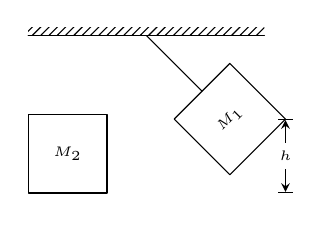
\begin{tikzpicture}[line cap = round, line join = round]
  \begin{scope}[xshift = -1cm]
    \block

    \node[font = \tiny] at (0, -1.5cm) {$M_2$};
  \end{scope}

  \begin{scope}[transform shape, rotate = 45]
    \draw (0, 0) -- (0, -1cm);
    \block

    \coordinate (P) at (0.5cm, -2cm);
    
    \node[font = \tiny] at (0, -1.5cm) {$M_1$};
  \end{scope}

  \draw (-1.5cm, 0) -- (1.5cm , 0);

  \path[name path = dline] (P) -- +(0, -1cm);
  \path[name path = vline] (0, -2cm) -- +(2cm, 0);
  \path[name intersections = {of = dline and vline, by = P1}];

  \draw[xshift = .1cm, >=stealth, |<->|] (P) -- (P1) node[font = \tiny,
  pos = 0.5, fill = white, inner sep = 0.1cm] {$h$}; 

  \fill[pattern = north east lines] (-1.5cm, 0) rectangle (1.5cm, 0.1cm);
\end{tikzpicture}
\end{document}
%%% Local Variables:
%%% mode: latex
%%% TeX-master: t
%%% End:
